
This section describes some of the main aspects of the software development
process and software lifecycle as specified in CENELEC EN 50128 and discusses
some potential issues with the implementation using agile methods like SCRUM.

In the openETCS proposal, it was decided to use the V-model for development
(V2.2 Section 3.4.3), as shown in CENELEC EN 50128 Figure~4

\begin{figure}[ht]
  \centering
  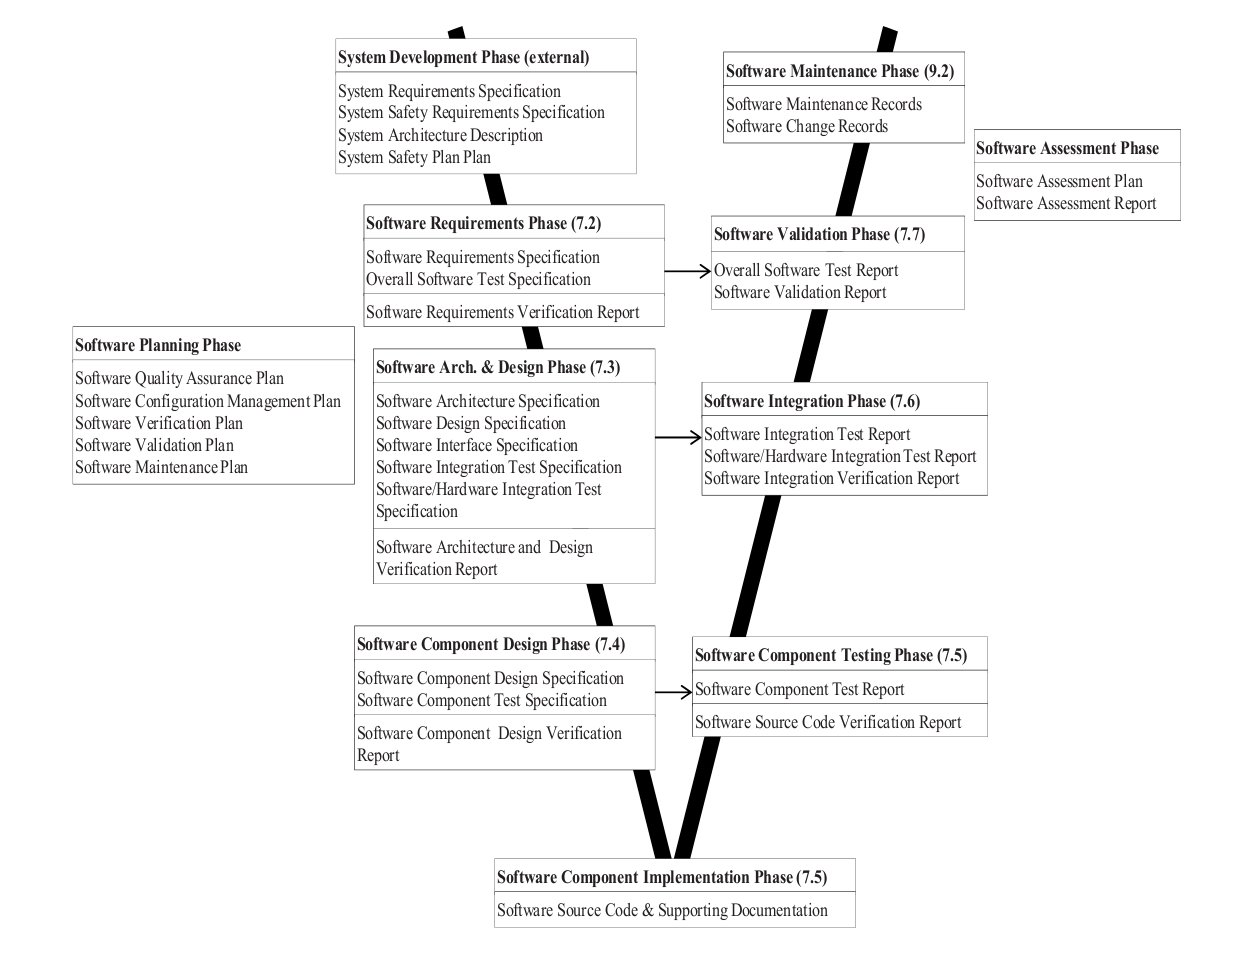
\includegraphics[width=.9\textwidth]{V-Model}
  \caption{General Development Lifecycle as in CENELEC}
  \label{fig:develop-lifecycle-cenelec}
\end{figure}

\subsection{Objectives}
\label{sec:objectives}

The two most important goals of the CENELEC EN 50128 standard are the separation
of the lifecycle into well-defined phases and to produce and record all
documentation of the development process. In addition, the standard specifies
some important constrains which must be fulfilled by a development
process. These constraints mainly result from the application in safety critical
domains.

Naturally, the document-centric nature and the additional constraints are not
necessarily fulfilled by generic software development processes which have been
developed for non-critical domains. In particular for agile development
processes like SCRUM, an adaptation in some aspects will be
required. In openETCS the development process will be less  focused on
extracting the real wishes from the client from user-stories, but on finding the
intended semantics of the ERTMS specification.

\subsection{Organisational Structure and Roles}
\label{sec:organ-struct-roles}

CENELEC EN 50128 defines a set of required roles for the development of SIL4 (or
SIL3) compliant software (e.g. requirements manager, assessor, etc., for a full
list see 5.1 of CENELEC EN 50128). Theses roles and which of these roles can be
filled by the same person are specified in 5.1.2.10 of the standard. This
distribution and in particular the required separation of several of the roles
will be mandatory for the development process.

\begin{figure}[ht]
  \centering
  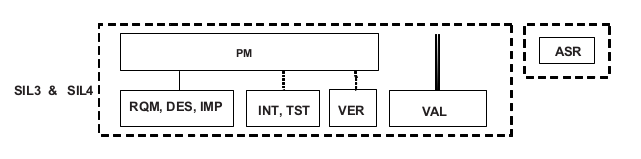
\includegraphics[width=\textwidth]{CenelecRoles}
  \caption{Preferred Organisational Roles}
  \label{fig:preferred-roles}
\end{figure}

Fig.~\ref{fig:preferred-roles} shows the preferred organisational structure
according to CENELEC EN 50128, in particular  the role separations,
e.g., the verifier cannot be the same person as tester, the requirements
manager must be a different person than the integrator and the validator must be
independent of the project manager.

In contrast, the SCRUM development process only defines three roles: project
owner, SCRUM master and team member. These roles mus be refined for an agile SW
development in accordance with the standard.

\subsection{Documentation}
\label{sec:documentation}

The development according to CENELEC EN 50128 is document-centered and many
mandatory documents mus be created. This is in contrast to the agile
development, where only the software is seen as the relevant product. So for
each of the small iterations of the agile process not only the SW shall be of
concern, but also the generated documentation, in particular the update of
existing documentation and the verification of consistency regarding related or
referenced documents.

\subsubsection{Consistency of Documentation}
\label{sec:cons-docum}

It is mandatory to have a consistent definition and usage of all terms,
abbreviations etc. This is especially important if the development process uses
small scale iterations, as the consistency must be assured and restores in
necessary after each iteration. In particular, it must be assured at all times,
that dependent documents, i.e., in hierarchical relation do not contradict each
other.

\subsubsection{Traceability of Requirements}
\label{sec:trac-requ}

For each of the generated documents, the traceability must be assured by
referencing all other concerned documents and by specifying unique reference
numbers. Just like consistency, this traceability is a very important aspect
which is often not a concern in more general software development processes.


\subsection{Quality Assurance}
\label{sec:quality-assurance}

The SW development according to CENELEC EN 50128 requires parallel quality
assurance procedures. This will be well implementable using agile development
which uses several techniques to assure the quality of the results. The test
driven approach and the unit tests used by agile methods, as well as techniques
for increasing code quality like continuous build and pair programming shall be
encouraged.

\subsection{Conclusion}
\label{sec:conclusion}

Some requirements of the CENELEC EN 50128 norm do not allow to apply an agile
software development process directly. Agile methods are conducted in close
cooperation with the client, they use ``user-stories'', work in very short
iteration and have only few required roles.

To use agile methods in safety critical development, the  process shall be
adapted to the requirements. The roles shall be defined differently, in
particular the necessary separation of roles, the user-stories shall be an
equivalent of he requirements of the SRS and all results of the short term
iterations must be verified for their consistency wrt. the documentation and the
documentation must be changed accordingly.




%% some ideas of agile in safety critical development:
%% see open-DO project, presentation Peter Gardner from AdaCore
%% www.open-do.org
%%

%%% Local Variables:
%%% mode: latex
%%% TeX-master: "wp-2.2"
%%% End:
